% !TEX root = ../thesis.tex

\chapter{Neural network training data}
\label{chap:neural-network-data}

Over their relatively brief existance, neural networks have been shown to perform increasingly impressive tasks (e.g.  \cite{openai2019dota}, \cite{openai2023gpt4}, 
and many more). However, they learn by example. The performance of a neural network is directly linked to the input data it receives during training. If the 
training data is not an accurate example of real world information a network later operates on, insight gained from it is at best an approximation, and at worst
completely randomly generated data. 

As such, it is not a question \textit{if} some neural network architecture can learn to identify an extensive air shower from WCD data, but rather which 
implementation, fed with which information, does. For this purpose, this chapter explains the procedure with which training data is generated. As stated above, this
must occur with a focus on being representative of data actually measured in the SD array. The elected approach to create time traces is modularized. The structure
of this chapter reflects this. First, general comments about the characteristics of background data (i.e. the WCD detector response in the absence of an extensive 
air shower) are made in \autoref{sec:background-dataset}. Next, the process to extract signal originating from CRs is detailed in \autoref{sec:signal-dataset}.
Lastly, building the time trace from the aforementioned modules and drawing samples from it for a neural network to train on is done in \autoref{sec:trace-building}
and \autoref{sec:sliding-window-analysis}.

\section{Background dataset}
\label{sec:background-dataset}

While a flux of partices causes elevated ADC levels in both the HG and LG channels of a WCD PMT during a shower event, the lack of such a phenomenon does not imply 
the readout information is uniformly flat. Instead, it hovers around the channels' baseline (c.f. \autoref{sec:surface-detector}) with occasional spikes upwards 
due to low-energy particles impinging on the detector. Coupled with electronic noise from the many digital components in the station electronics, the 
\textbf{U}pgraded \textbf{U}nified \textbf{B}oard (UUB), this constitutes the data that is collected inbetween air shower events.

\subsection{Accidental muons}
\label{ssec:accidental-muons}

Most low-energy background particles present in the detector are muons. These are produced in the upper atmosphere during cascading processes analog to 
\autoref{chap:physical-background}. Due to the low primary energy the electromagnetic component of the shower is thermalized before it reaches surface level. The 
muonic component by itself does not contain enough information to enable an accurate reconstruction of primary energy and origin. This fact, coupled with the high
flux of events at lower energies ($\Upphi|_{E=\SI{100}{\giga\electronvolt}} \approx \SI[per-mode=power]{1}{\per\meter\per\second}$ \cite{boezio2000measurement}) 
make these events unsuitable for analysis. Stray muons, even though they originate from extensive air showers, must consequently be considered background events.

The rate at which such particles traverse a WCD tank is $f_\text{Acc.}\approx\SI{4.665}{\kilo\hertz}$ \cite{DavidBackgroundSim}. Their arrival time is 
Poisson-distributed. This implies that generally, one in 14 time traces contains signal from a low-energy background event. Coincidences of two accidental 
muons occur on a sub-percent level. Any higher order of coincidences is likely originating from a single air shower process. The typical signal recorded by the 
surface detector from a single muon is presented in \autoref{fig:muon-response}.

\begin{figure}
	\centering
	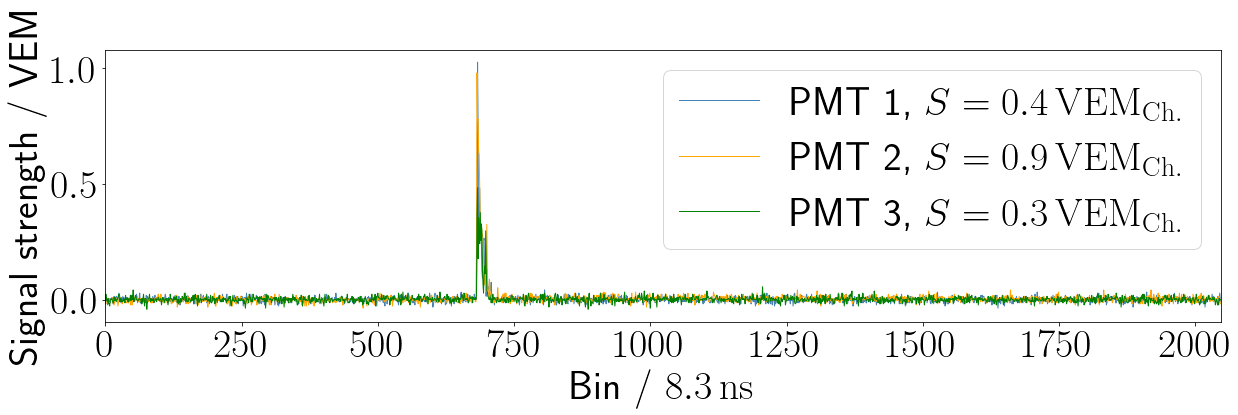
\includegraphics[width=0.8\textwidth]{./plots/muon_response.png}
	\caption{The simulated time trace from a single muon. The maximum peak of the time trace is equal to \SI{1}{\Peak}. The integral over each PMT, $S$, sums to
    $\approx\SI{1}{\Charge}$.}
	\label{fig:muon-response}
\end{figure}

A library of background traces of this type was provided by David Schmidt \cite{DavidBackgroundSim}. However, only the largest response of the three WCD PMTs is
available for this library. Due to the lack of information one is either forced to assume the response to a low-energy background particle is the same across all 
PMTs, or neglect the response of the two remaining PMTs altogether upon injectiong a background muon into a signal trace (c.f. \autoref{sec:trace-building}). In 
both cases, neural networks are provided an easily detectable pattern to discern such particles from "real" shower signal. As a result, it should be refrained 
from training AI triggers on this dataset.

\subsection{Electronic noise}
\label{ssec:electronic-noise}

Electronic noise is the umbrella term given to the distortions that some signal is subject to during digital readout. Such noise can have many different origins.
An illustrative example is given by the \textbf{L}aser \textbf{I}nterferometer \textbf{G}ravitational wave \textbf{O}bservatory, which excludes the \SI{60}{\hertz}
band and its' harmonics from analysis. This is owed to the fact that the DC frequency standard in the United States introduces systematic uncertainties in the
detector \cite{martynov2016sensitivity}. In the electronics of Pierre Augers' SD array, electronic noise is assumed to be Gaussian. That is to say that the 
\SI{}{\ADC} values of a time trace that was measured while no particle produced signal in the tank are normally distributed around the baseline. The standard 
deviation can be estimated from monitoring data, as is shown in \autoref{fig:random-traces}.

\subsection{Random traces}
\label{ssec:random-traces}

Both above mentioned phenomena can be simulated, and the simulation results used as background training data for the neural networks discussed in the next chapter.
A more accurate method however, and the approach elected for this work is to utilize directly measured data from the field. Thanks to the work of David Nitz, there 
exist collections of so called random-traces\footnote{to avoid possible confusion between this dataset and a \textit{random} trace in the statistical sense, the 
traces recorded by David Nitz are referred to as random-trace, with a hypen.} that were gathered by forcing DAQ readout via a manually set trigger. 

In particular, two datasets of UUB random-traces have been created until now. They were taken from 13th-18th March 2022, and 14th-18th November 2022 respectively. 
The first set contains data a total of sixteen million time traces distributed over four different SD stations. For reasons explained in 
\autoref{ssec:random-trace-calibration}, only data from the first set is used in the analysis presented in this work.

\subsubsection{Characteristics}
\label{ssec:random-trace-characteristics}

Contrary to the naming of the random trigger, it occurs at a deterministic time. More accurately, the process of measuring random-traces is as follows;
A single time trace ($2048\cdot\SI{8.333}{\nano\second} = \SI{17.07}{\micro\second}$) is written to the local station buffer every $\SI{10}{\milli\second}$. Once
the buffer has accumulated enough data, it is written to a USB storage device. Because of a bottleneck in the last step, the process takes about \SI{22}{\hour}
per station \cite{nitzCorrespondence}.

It is thus not the trigger that is unpredictable, but the data measured by each trigger. Due to the read/write process being indepentant of the measured data
(as opposed to the algorithms in \autoref{chap:classical-triggers}) the latter must be considered to be essentially random. For the most part, random-traces are 
assumed to consist solely of electronic noise. However, signal of cosmic origin - be it accidental muons or extensive air showers - will appear in the data at a
rate at least consistent with \autoref{sec:classical-triggers-performance}.

A crude analysis of the type of noise in the random-traces can be made by examining the spectral density of the dataset, shown in \autoref{fig:random-traces}.
Harmonic modulations visible in both spectra might originate from an offset between last and first bin of the random-traces. If this offset is nonzero, the 
periodic extension of $f(x)$ exerts a step-function-like behaviour. The Fourier transform consequently reflects this \cite{burrows1990fourier}. Still, several
features of $| \hat{f}(\xi) | ^{2}$, espically present at $\SI{10}{\mega\hertz}$, imply the presence of systematic noise in the UUB. Nevertheless, the large scale 
form of the spectral density is compatible with at least two noise models, that cannot be distinguished based on the data at hand:

\begin{itemize}
	\item  $\mathbf{| \hat{f}(\xi) | ^{2} \propto \exp\left(\frac{(\xi - \mu)^2}{2\sigma^2}\right)}$. The spectral density is Gaussian. This implies the noise is 
	Gaussian distributed as well, confirming the assumption in \autoref{ssec:electronic-noise}.
	\item $\mathbf{| \hat{f}(\xi) | ^{2} \propto} \exp\left(-m\xi + b\right)$. The spectral density is proportional to $\xi^{-n}$ for some power $n$. The case 
    $n = 2$ ($\SI[per-mode=symbol]{-6}{\deci\bel\per\octave}$ attenuation) seems to describe the observations well, hinting that the generating function could be 
    Brownian.

\end{itemize}

\begin{figure}
	\centering
	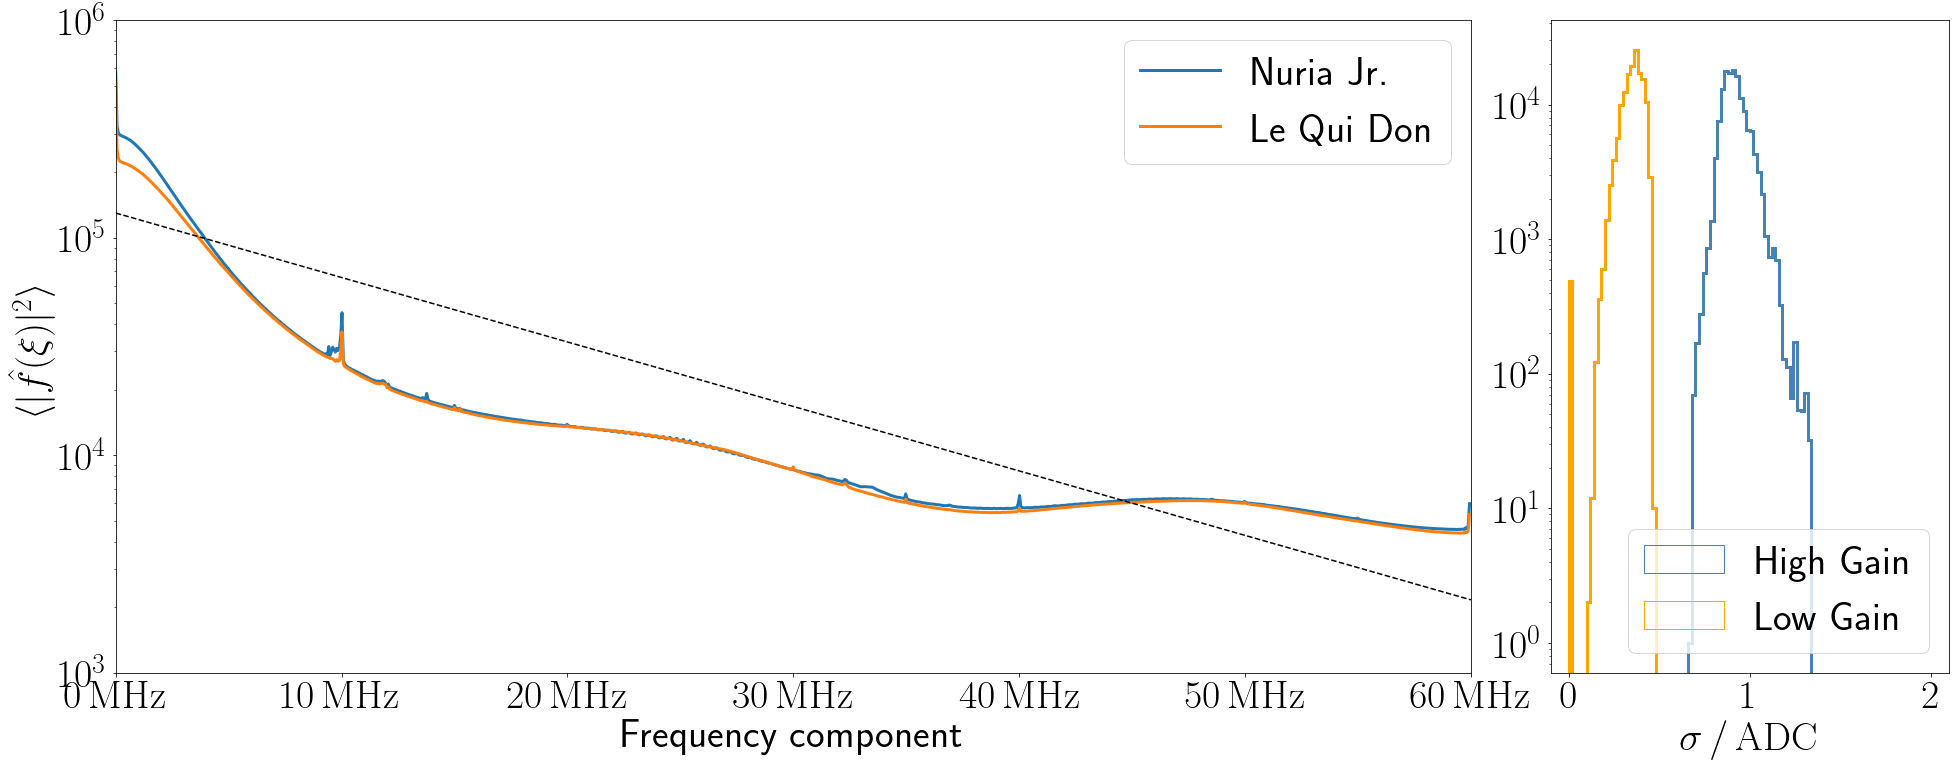
\includegraphics[width=0.8\textwidth]{./plots/fft_variance_plot_combined.png}
	\caption{(\textit{Left}) The random-trace spectral density for two stations. Plotted with a dashed black line is reference attenuation curve falling at 
	$\SI[per-mode=symbol]{-6}{\deci\bel\per\octave}$. The spike at \SI{10}{\mega\hertz} is of unknown origin and represents systematic noise in the UUB 
	electronics. (\textit{Right}) Example variance of all UUB stations in the surface detector array. The data shown in this plot was recorded on November 15th 
    2022.}
	\label{fig:random-traces}
\end{figure}

\subsubsection{Calibration}
\label{ssec:random-trace-calibration}

The random-trace files contain raw measurement data in units of $\SI{}{\ADC}$ for the HG and LG channel of the three WCD PMTs. In a first step to standardize this
information, the baseline is substracted from each FADC bin. This is done via the baseline finding algorithm described in \autoref{ssec:offline-calibration} and 
\cite{tobiasBaseline, tobiasBaselineUUB}. Note that this approach differs from the baseline finding algorithm that runs on each station (c.f. 
\autoref{ssec:online-calibration}). However, the difference is negligible ($<<\,\SI{1}{\ADC}$) for traces that do not contain any signal, which is the case for the 
vast majority of the dataset.

Next, the baseline-substracted time traces are converted from units of $\SI{}{\ADC}$ to $\SI{}{\Peak}$. This conversion is not straight forward, as it requires 
knowledge of \Ipeak at the time of data taking. Each station estimates this value in periodic time intervals in the context of monitoring diagnostics.

For the second dataset of random-traces (taken from 14th-18th November 2022) a UNIX timestamp packaged with each time trace may be related to monitoring data. This 
reveals that no information regarding \Ipeak was forwarded to CDAS for any station while it recorded random-traces. As a result, the entire dataset is unfortunately 
rendered useless for this work.

For the first collection of random-traces, monitoring data is available, but there exists no timing information for the individual traces. Only the date of the 
measurement is known. The elected procedure to evaluate data as accurately as possible is thus to calculate the day average of \Ipeak and \Qpeak and take this as 
the best (first) estimate for each trace. As can be seen in \autoref{fig:random-trace-diagnostics}, this eliminates half of the remaining dataset, as two of the four 
stations show a large variance in \Ipeak. The day average in these particular cases is not a good estimator for calibration purposes. For this reason, only random 
traces from the stations Nuria and Le Qui Don, measured in the March dataset are used for analysis purposes, as their $I_\text{VEM, Rand.}$ is stable.

As a crosscheck to verify the goodness of the approximation, the T2 trigger rate as reported by the calibration process is related to the trigger rate obtained by
direct calculation over all (calibrated) random-traces. By extension, this also serves as a unit test for the classical triggers as they will be implemented in 
\autoref{chap:classical-triggers}. The results of this analysis are shown in \autoref{fig:random-traces-correction}. As is clear from the plot, the rates 
calculated from the two different approaches are not in accordance. This indicates systematic errors in the calibration (a wrong implementation of trigger 
algorithms is disfavoured from the discussion in \autoref{chap:classical-triggers}). The errors are consistent across both considered stations. It is found that 
calculated trigger frequencies are $\approx25\%$ lower than what is taken from monitoring. It is unclear why this discrepancy occurs, as it implies that the 
stations do not use the same threshold values for triggering as they report.

In any case, $I_\text{VEM, Rand.}$ must be adjusted to reflect this. A $25\%$ increase in trigger rate is relatable to a $\approx10\%$ decrease in \Ipeak. The 
calibration scaling factors for random-traces thus become the values listed in \autoref{tab:I-peak-random}.

\begin{table}
	\begin{center}
	\caption{Calibration constant \Ipeak for random-traces.}
	\begin{tabular*}{0.6\textwidth}{@{\extracolsep{\fill}} c|c|c}
		\toprule
		PMT \# & Nuria & Le Qui Don \\
		\midrule
		1 & \SI{159.34}{\ADC} & \SI{145.79}{\ADC} \\
		2 & \SI{161.37}{\ADC} & \SI{144.63}{\ADC} \\
		3 & \SI{149.91}{\ADC} & \SI{154.62}{\ADC}
	\label{tab:trigger-thresholds}
	\end{tabular*}
	\end{center}
\end{table}

\begin{figure}
	\centering
	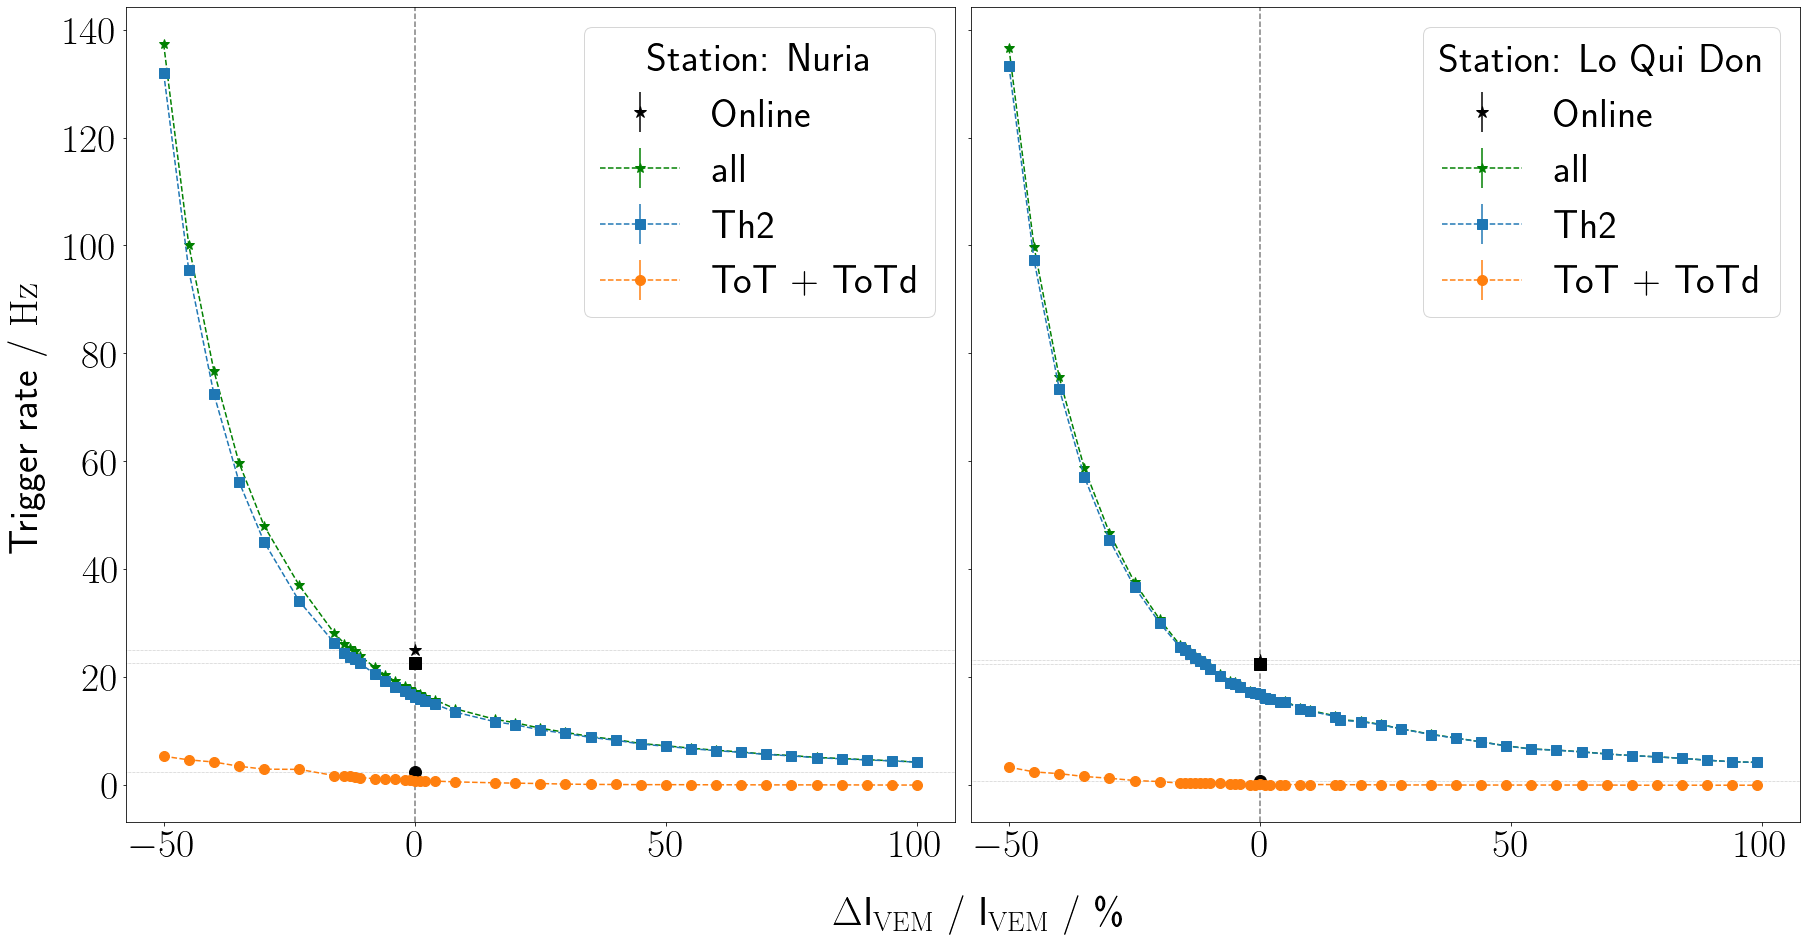
\includegraphics[width=\textwidth]{./plots/random_traces_correction_factor.png}
	\caption{The online reported T2 trigger rate (black) does not match the calculated trigger rate. Only a decrease $\Delta$\Ipeak by $1/10$th of the original 
	\Ipeak gives a close approximation of the observed rate when manually calculating trigger frequencies.}
	\label{fig:random-traces-correction}
\end{figure}

\begin{landscape}
    \begin{figure*}
        \centering
        \begin{subfigure}[b]{0.5\textwidth}
			\hspace{-4cm}
            \centering
            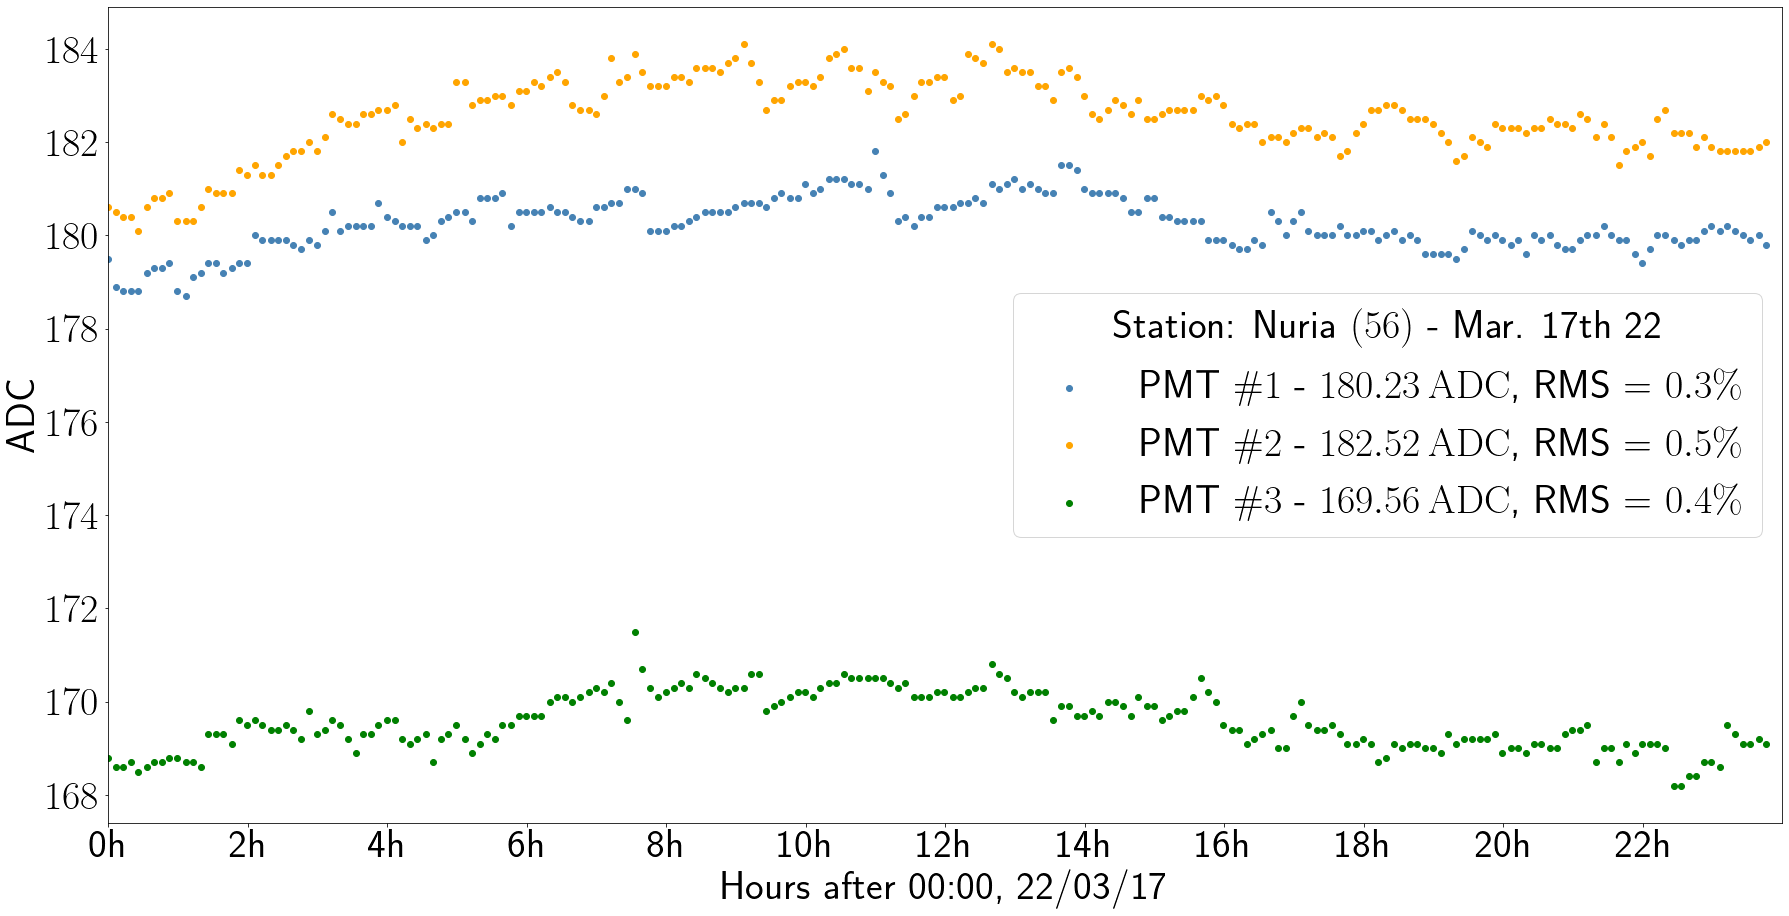
\includegraphics[width=0.7\textheight]{./plots/random_trace_diagnostics_nuria.png}
        \end{subfigure}
        % \hfill
        \begin{subfigure}[b]{0.5\textwidth}  
            \centering 
            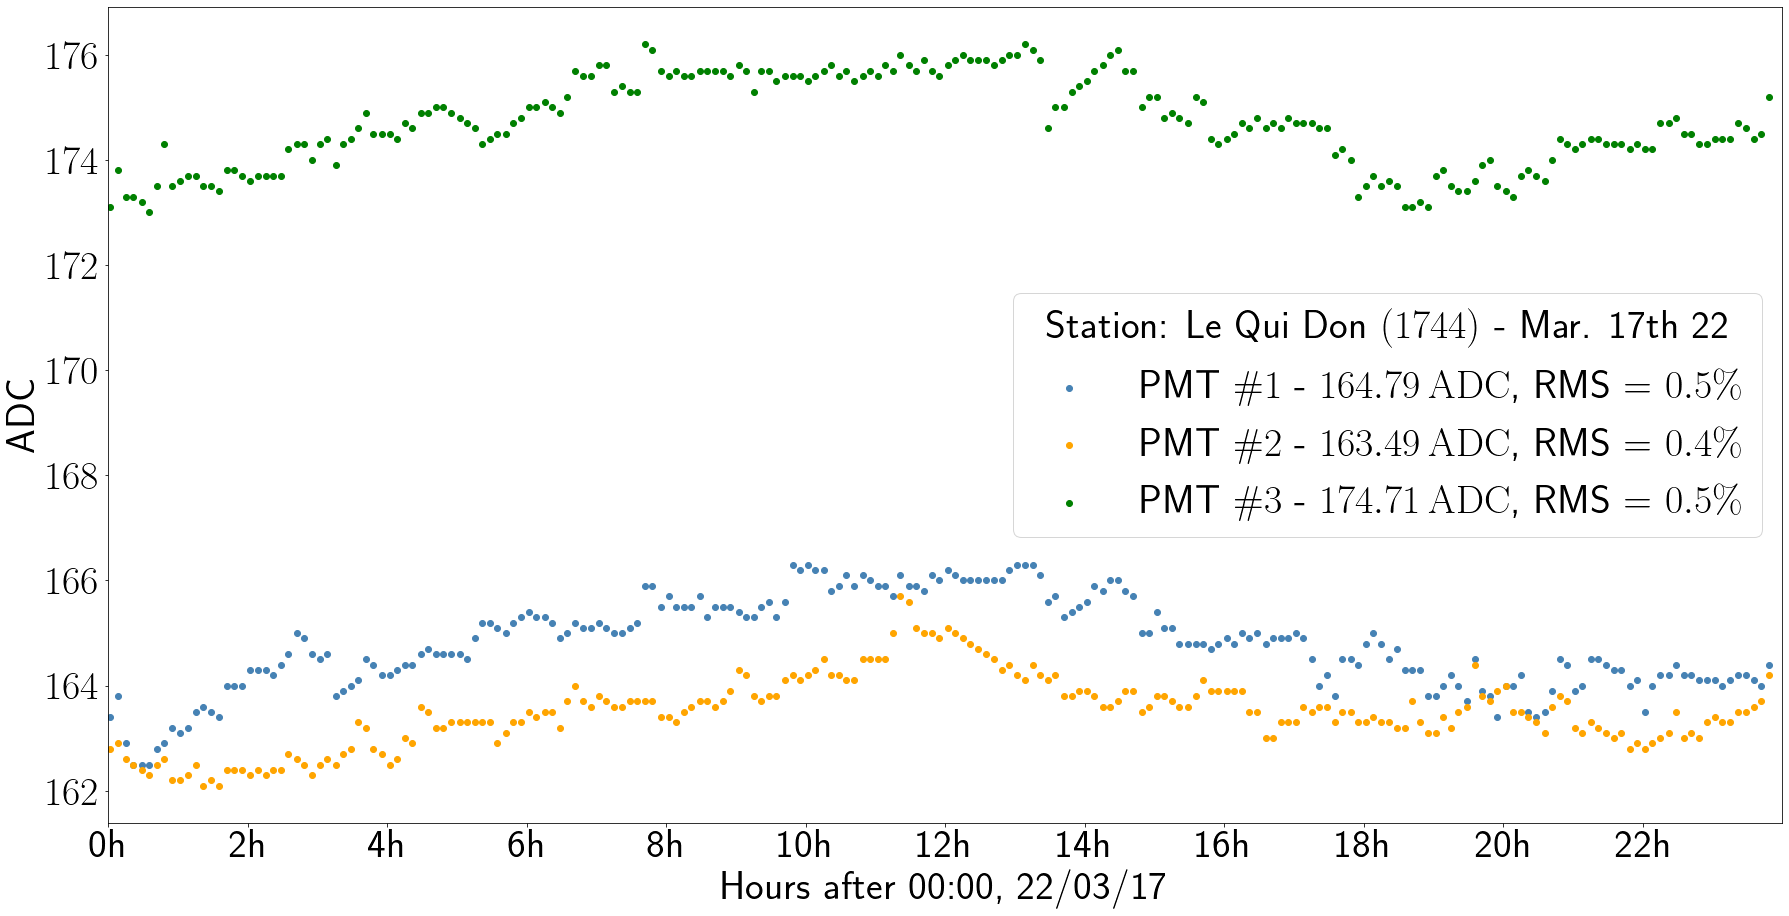
\includegraphics[width=0.7\textheight]{./plots/random_trace_diagnostics_le_qui_don.png}
        \end{subfigure}
        \vskip\baselineskip
        \begin{subfigure}[b]{0.5\textwidth}
			\hspace{-4cm} 
            \centering 
            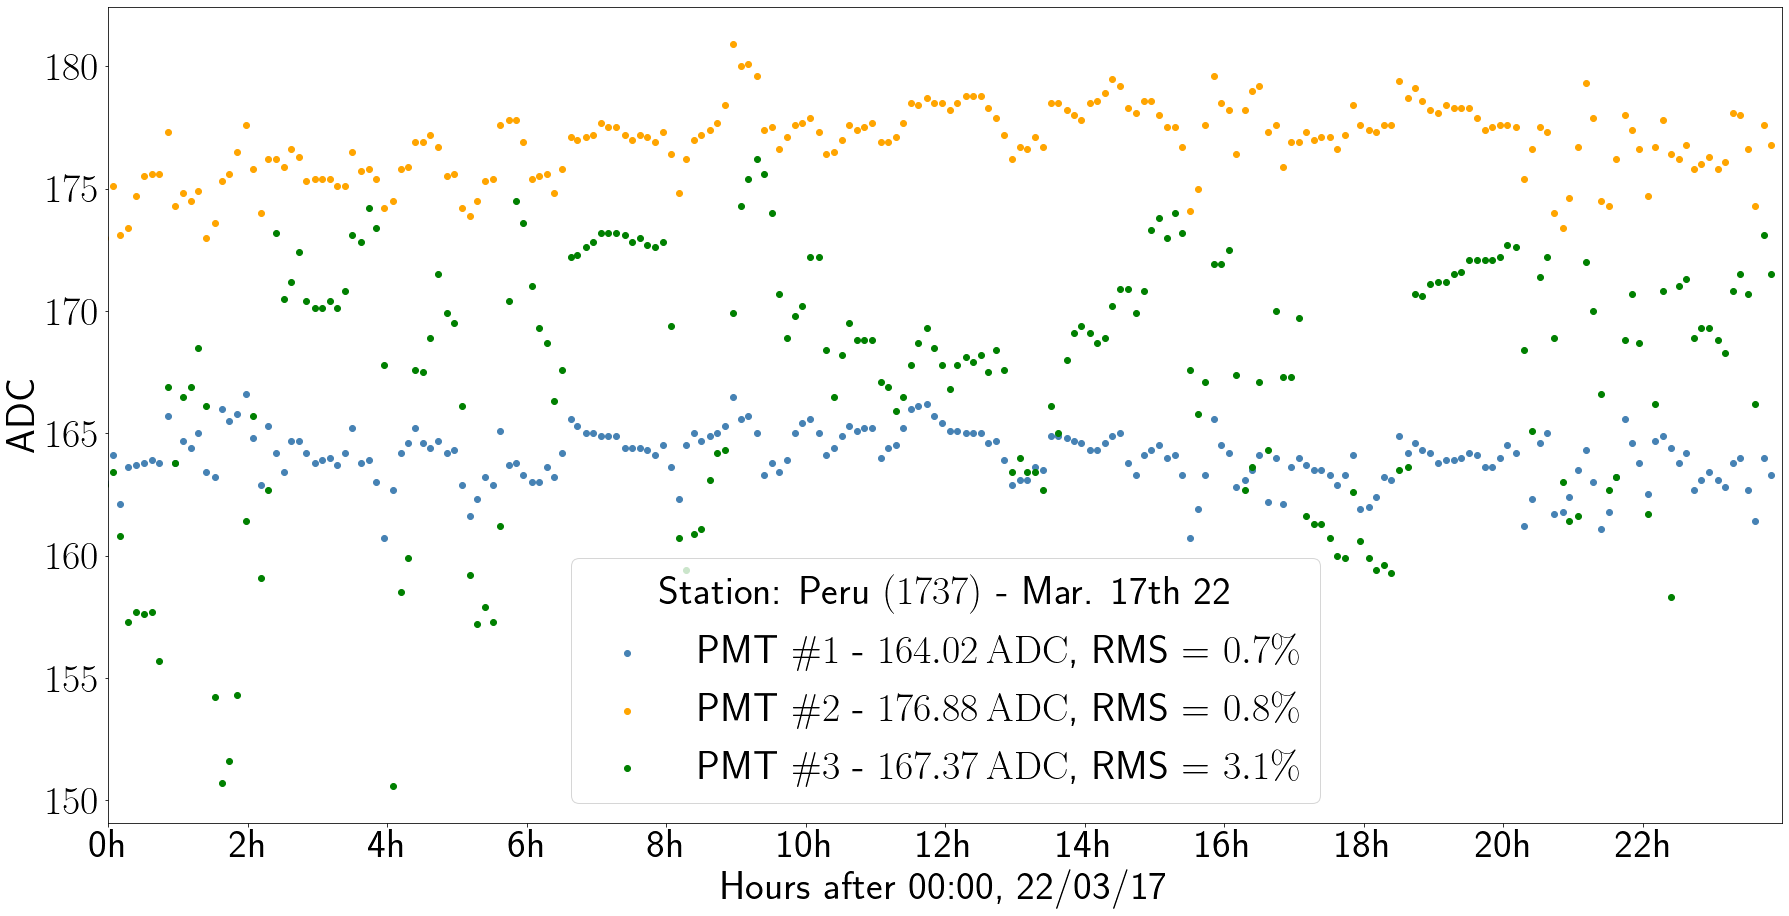
\includegraphics[width=0.7\textheight]{./plots/random_trace_diagnostics_peru.png}
        \end{subfigure}
        % \hfill
        \begin{subfigure}[b]{0.5\textwidth}   
            \centering 
            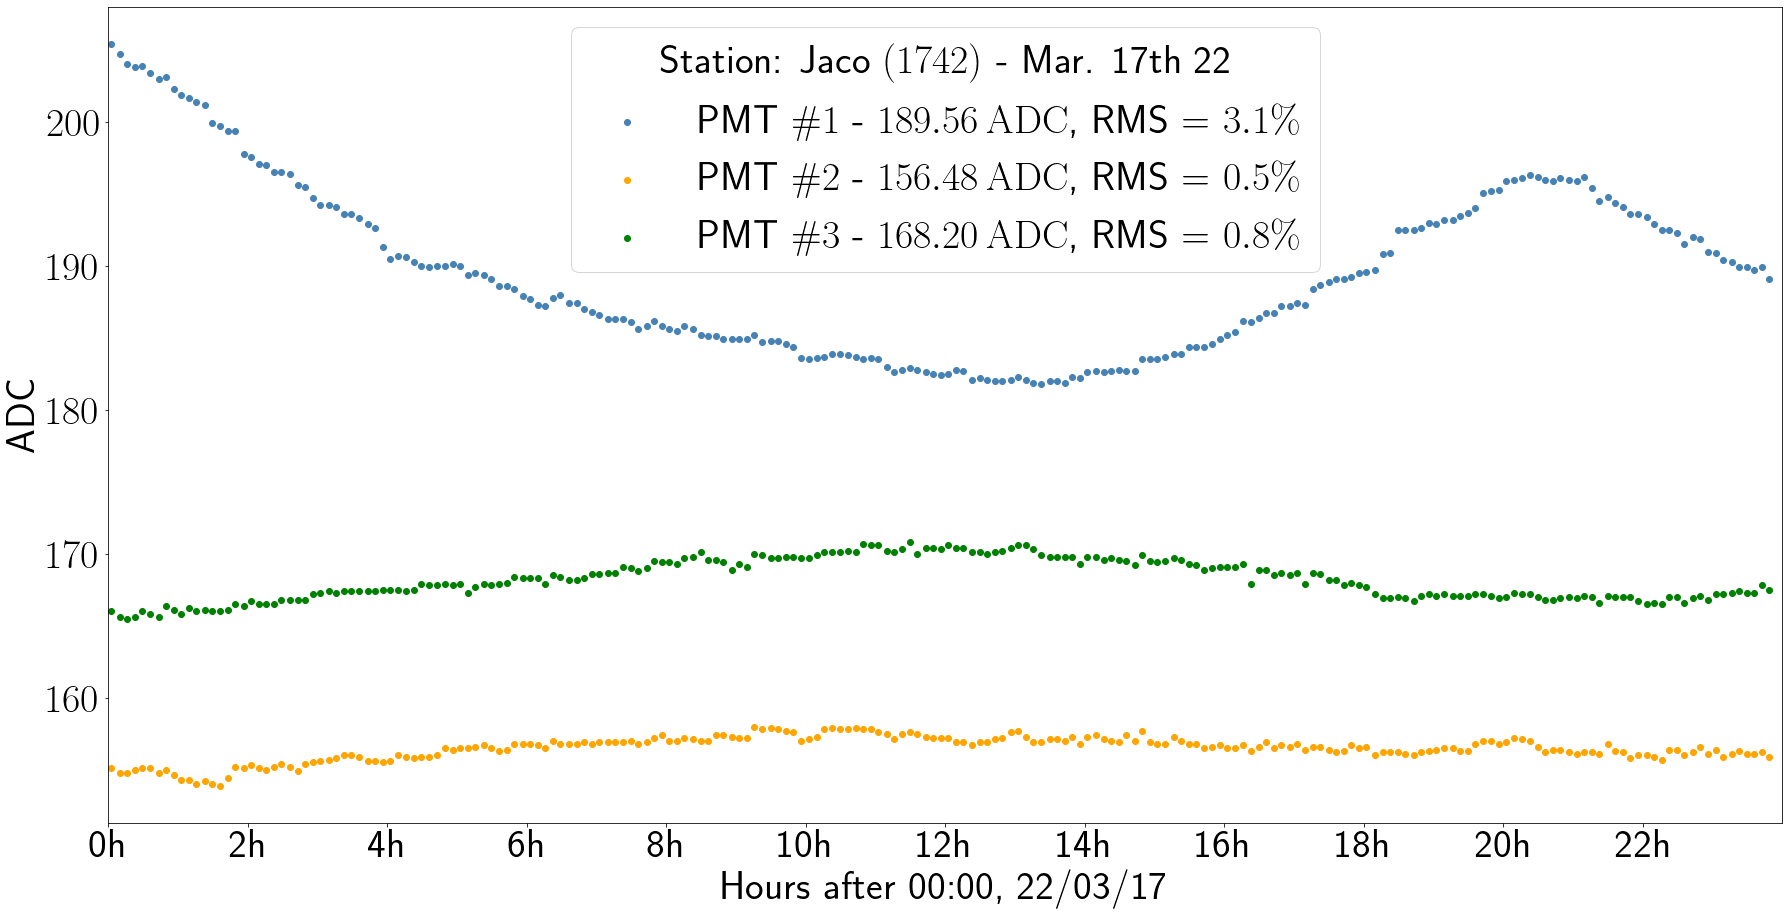
\includegraphics[width=0.7\textheight]{./plots/random_trace_diagnostics_jaco.png}
        \end{subfigure}
        \caption{Monitoring values for the four stations available in the random-trace dataset measured in March '22. The bottom two stations show a large variance
		in \Ipeak for at least one PMT. The two stations in the first row (Nuria, Le Qui Don) are more stable ($\sigma\,/\,\mu < 1\%$).} 
        \label{fig:random-trace-diagnostics}
    \end{figure*}
\end{landscape}

\section{Signal dataset}
\label{sec:signal-dataset}

In the context of this work, a "signal" (as opposed to background) is \textit{any} detector response caused by extensive air showers. Admittedly, this choice of 
classification is not ideal, as the particle density far from the shower axis grows sparse. Time traces recorded at those locations look very similar to ones 
raised by accidental muons. In any case, ramifications and possible solutions to this problem are further discussed in the following chapters. 

In order to isolate the signal stemming from shower particles only, an \Offline simulation using Geant4 is executed on CORSIKA source files \cite{heck1998corsika}.
These are a total of $40557$ simulated showers with a proton primary of energy $16 < \log\left(E/\SI{}{\electronvolt}\right) < 19.5$.  All showers are simulated 
using the hadronic interaction model QGSJET-II.04 \cite{ostapchenko2007status}.

In the process, the electronic feedback of the WCD PMTs is evaluated without any disturbance factor (see \autoref{sec:background-dataset}). That is to say that 
the time trace obtained from such simulations is identically zero (in units of \SI{}{\ADC}) at any point in time where no ionizing particles are present in the WCD. 
An example trace that visualizes this is shown in \autoref{fig:component_adding}. Next, the trigger conditions both for individual stations and on the event-level 
are altered to trigger on everything. This step is needed in order to save all traces to the simulation output, an \textbf{A}dvanced \textbf{D}ata \textbf{S}ummary 
\textbf{T}ree (ADST). If this was not the case, only traces that already satisfy current trigger conditions would be written to disk. A neural network training on 
such data could therefore at best be as efficient as the current triggers.

The choice of this approach forces some detours in the ADST readout. Instead of extracting the VEM calibrated traces directly, individual component traces, i.e. 
the PMT signal caused by muons, electrons and photons individually are summed to yield a total \SI{}{\ADC} trace. Signal stemming from hadrons or other components 
in the cascade is neglected. This does not impose any errors in the analysis, as the hadronic component espically lays close to the shower core, where the EM- and 
muonic component of the shower alone should already enable easy detection. Finally, the total trace as calculated above is extracted to a more easily accessible data 
format alongside shower metadata like primary energy, zenith, but also SPD, and particle count in the station the trace was recorded from.

\section{Trace building}
\label{sec:trace-building}

With the componentwise traces at hand, the total trace as would be recorded in the WCD PMTs for a given event, can be constructed. First, a trace container with 
default UUB trace length ($2048\,\text{bins}\cdot8.3\,\mathrm{ns}\,/\,\text{bin}=\SI{17.07}{\micro\second}$) and three components per bin (the three WCD PMTs) is 
initialized with all values equal to zero. Next, an arbitrary random-trace is selected as baseline. Since the FPGAs fundamentally count in the integer domain, the 
\SI{}{\ADC} data in the random-trace contains only whole numbers. As is, this wouldn't correctly model rollover when adding integer random-traces to floating point
simulation information. There two \SI{}{ADC} signals by themself might not exceed the threshold to cross to the next higher value, but the sum would; 
$\lfloor \SI{0.7}{\ADC} \rfloor + \lfloor \SI{0.4}{\ADC} \rfloor = \SI{0}{\ADC} \neq \SI{1}{\ADC} = \lfloor \SI{0.7}{\ADC} + \SI{0.4}{\ADC} \rfloor$. To account 
for this, uniformly distributed random numbers from 0 (inclusive) to 1 (exclusive)are added to the random-trace. 

Furthermore the $I_\text{VEM, Rand.}$ from random-traces (c.f. \autoref{ssec:random-traces}) will in general be different from \Ipeak simulated by 
\Offline ($I_\text{VEM, Off.} = \SI{215.781}{\ADC}$ compare \cite{offlineSource}). Thus the random-trace must be scaled by a factor 
$\frac{I_\text{VEM, Off.}}{I_\text{VEM, Rand.}}$ before being added to the container. 

If desired, accidental muons can be added to the trace container as well. This is done either by directly specifying a number of random injections, or throwing the
dice according to the injection frequency specified in \autoref{ssec:accidental-muons}. If the number of accidental muons is nonzero, a sample of random background
traces from \cite{DavidBackgroundSim} is drawn and each sample added to every PMT at a random uniform position somewhere in the trace. 
\autoref{fig:component_adding} shows an example where five muons are injected into the trace.

Last, the actual shower signal is added to the trace container. In principle, it can be added at any random position, similar to the random injections. However, for 
continuity reasons and ease of comparing to plots generated with other software, the latch bin for signal insertion is hardcoded to be the same as in \Offline, 
bin $660$. Since otherwise the data is in the correct $\SI{}{\ADC}$ format, no further manipulation of the data is necessary.

The trace container now holds all necessary components together, but remains in units of \SI{}{\ADC}. To convert to \SI{}{\Peak}, each bin in each PMT trace is 
floored to mimic the FPGA digital counting, and divided by the appropriate scaling factor \Ipeak. If traces need to be UB compatible the trace must be filtered and
downsampled in an intermediate step. This influences the scaling factor $I_\text{VEM, compat.}$ in a major way (compare \autoref{ssec:filtering-and-downsampling}). 
If the so-called full-bandwidth, UUB time trace is analyzed, the appropriate factor becomes $I_\text{VEM, Off.}$.

\begin{figure}
	\centering
	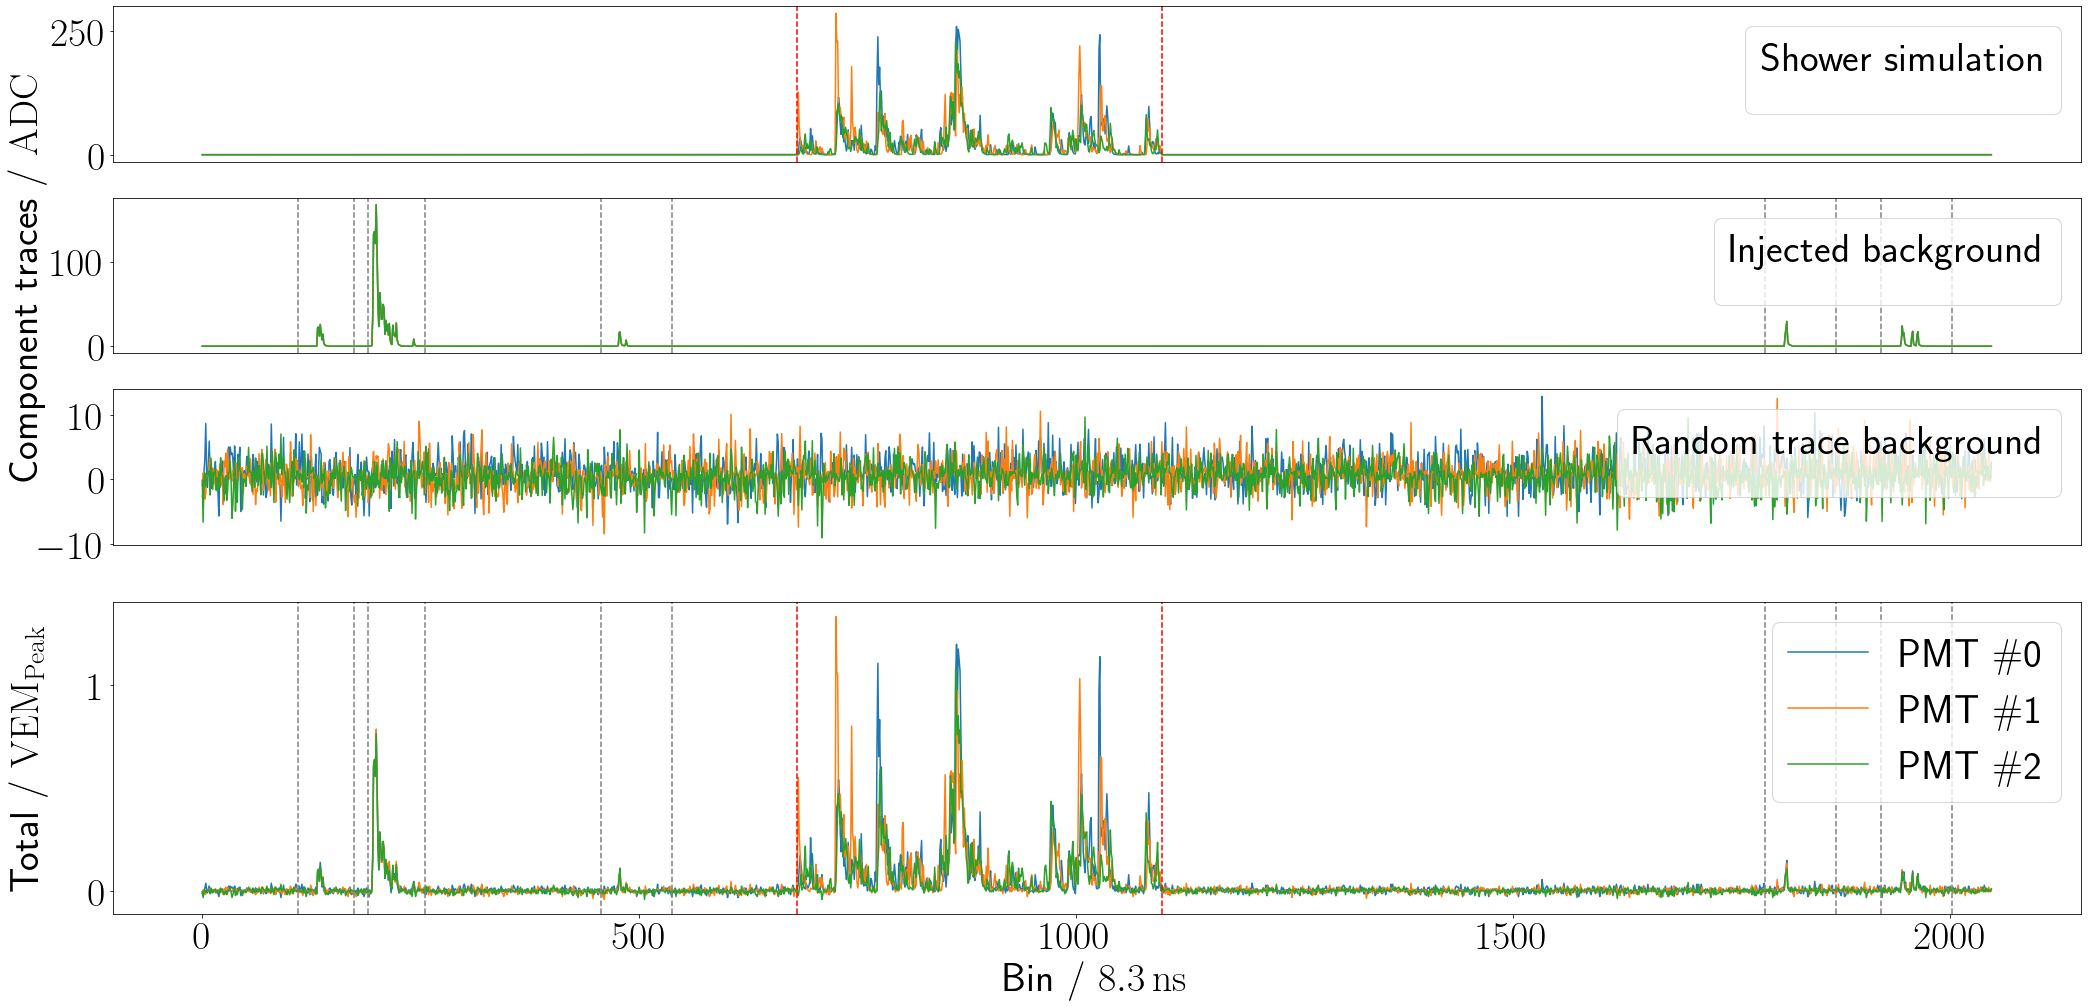
\includegraphics[width=\textwidth]{./plots/component_adding.png}
	\caption{The individual component traces (in units of \SI{}{\ADC}, top three plots) make up the eventual VEM trace (in \SI{}{\Peak}, bottom plot). The dashed 
    red (gray) lines signify where in the time trace the shower signal (injected muon signal) is located.}
	\label{fig:component_adding}
\end{figure}

\subsection{Filtering and downsampling}
\label{ssec:filtering-and-downsampling}

Altough the triggers discussed in the next chapter are meant to function completely autonomously in the SD field, their implementation requires some prior 
knowledge of the signal one desires to detect. For their use in the Auger observatory, several hyperparameters such as the thresholds of the Th-Trigger, or the 
window size of the ToT-trigger have been determined in studies (\cite{bertou2006calibration}, \cite{triggerSettings}, \cite{ToTtriggerSetting}). 

These studies were conducted using the predecessor, the \textbf{U}nified \textbf{B}oard (UB), of the hardware that is being installed during the AugerPrime upgrade
of the observatory. Most importantly, the UUB has a sampling rate that is three times larger (\SI{120}{\mega\hertz}) than that of UB electronics 
(\SI{40}{\mega\hertz}). Not only does this raise the number of bins in a standard time trace from 682 to $2^{11} = 2048$, but also drastically reduces the 
efficiency (in particular for ToT-like triggers) of the above discussed algorithms. Whereas a new  bin is measured every \SI{25}{\nano\second} in a UB station, the
triggers would receive a new input every $\approx\SI{8.3}{\nano\second}$ in a UUB setting.

The modus operandi elected by the Pierre Auger collaboration to circumvent this problem is to emulate UB electronics using the UUB electronics. This means that 
measured FADC bins are to be filtered and downsampled before any trigger runs over them. Software implementations by which this is achieved are listed in 
\autoref{app:filter-and-downsample}. The effect the filtering and downsampling has on measured data is visualized in \autoref{fig:uub-ub-comparison}.

While the features of the time trace largely remain intact, the absolute signal strength decreases due to a smearing effect imposed by the filtering. Overall, this
amounts to a $30\%$ difference in amplitude between UUB full-bandwidth traces and their filtered and downsampled counterpart. Since both measurements are derived 
from the same signal in the WCD though, this implies that \Ipeak must be adjusted by $~30\%$ as well, if traces are to be downsampled. This results in a 
compatibility scaling factor $I_\text{VEM, compat.} = \SI{163.235}{\ADC}$ \cite{OfflineSource}.

Recent contributions within the Auger collaboration (\cite{nitzTriggers, quentinComparison}), and to some extent also this work have shown that issues arise in the 
comparison of \textbf{L}ateral \textbf{T}rigger \textbf{P}robabilities (LTPs) that are run in this compatibility mode. Namely, the UUB trigger efficiency (where 
full-bandwidth traces are filtered and downsampled) is lower than that of UB stations. This implies that the filtering and downsampling algorithms in 
\autoref{app:filter-and-downsample} either make imprecise assumptions about the station electronics, or $I_\text{VEM, compat.}$ or the trigger thresholds 
themselves need to be adjusted further. This fact has to be kept in mind when discussing results and comparing lateral trigger probabilites from classical triggers
and neural networks. 

\begin{figure}
	\begin{subfigure}[b]{0.5\textwidth}
		\centering
		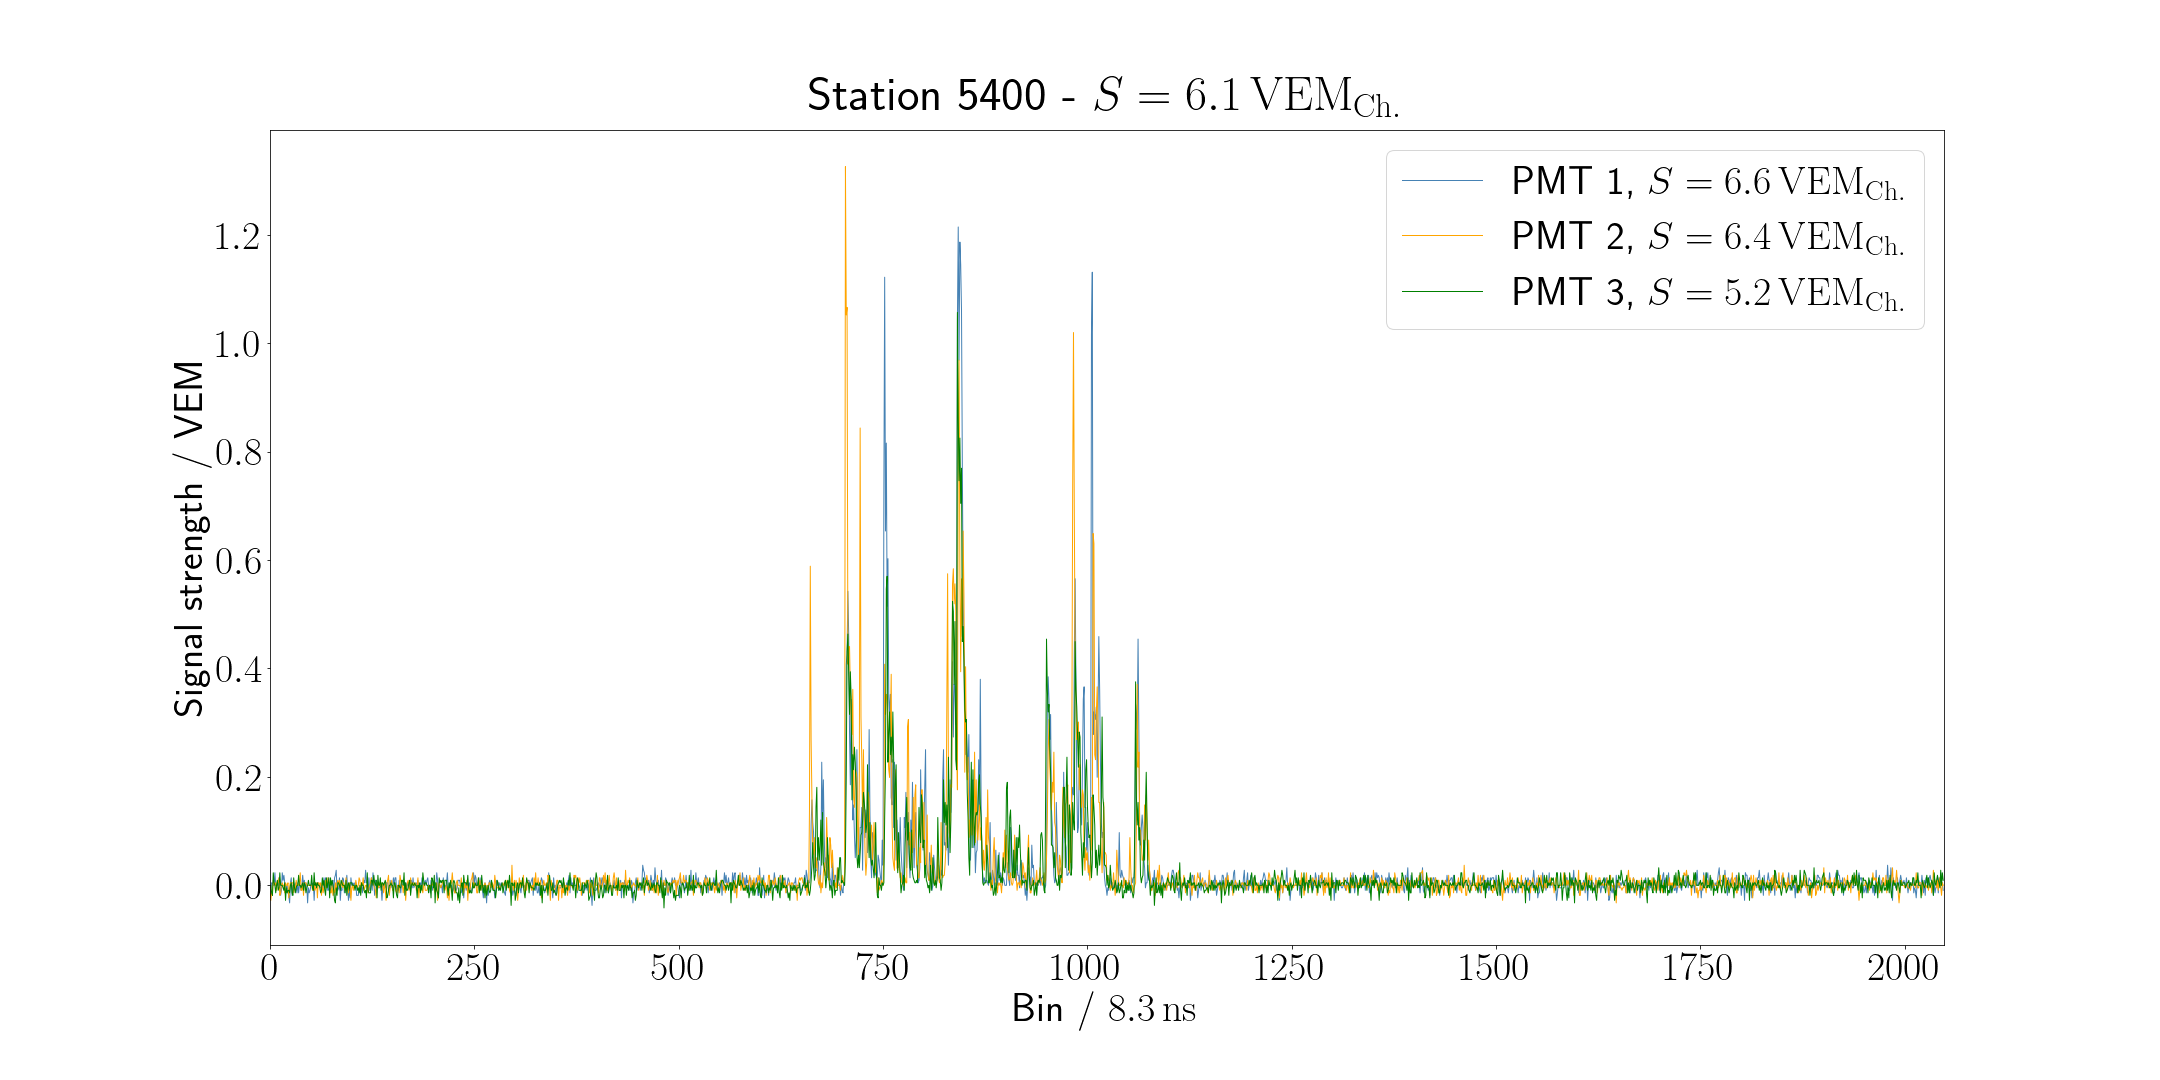
\includegraphics[width=\textwidth]{./plots/time_trace_UUB.png}
		\caption{\textbf{UUB time trace}}
		\label{fig:uub-time-trace}
	\end{subfigure}
	\hfill
	\begin{subfigure}[b]{0.5\textwidth}
		\centering
		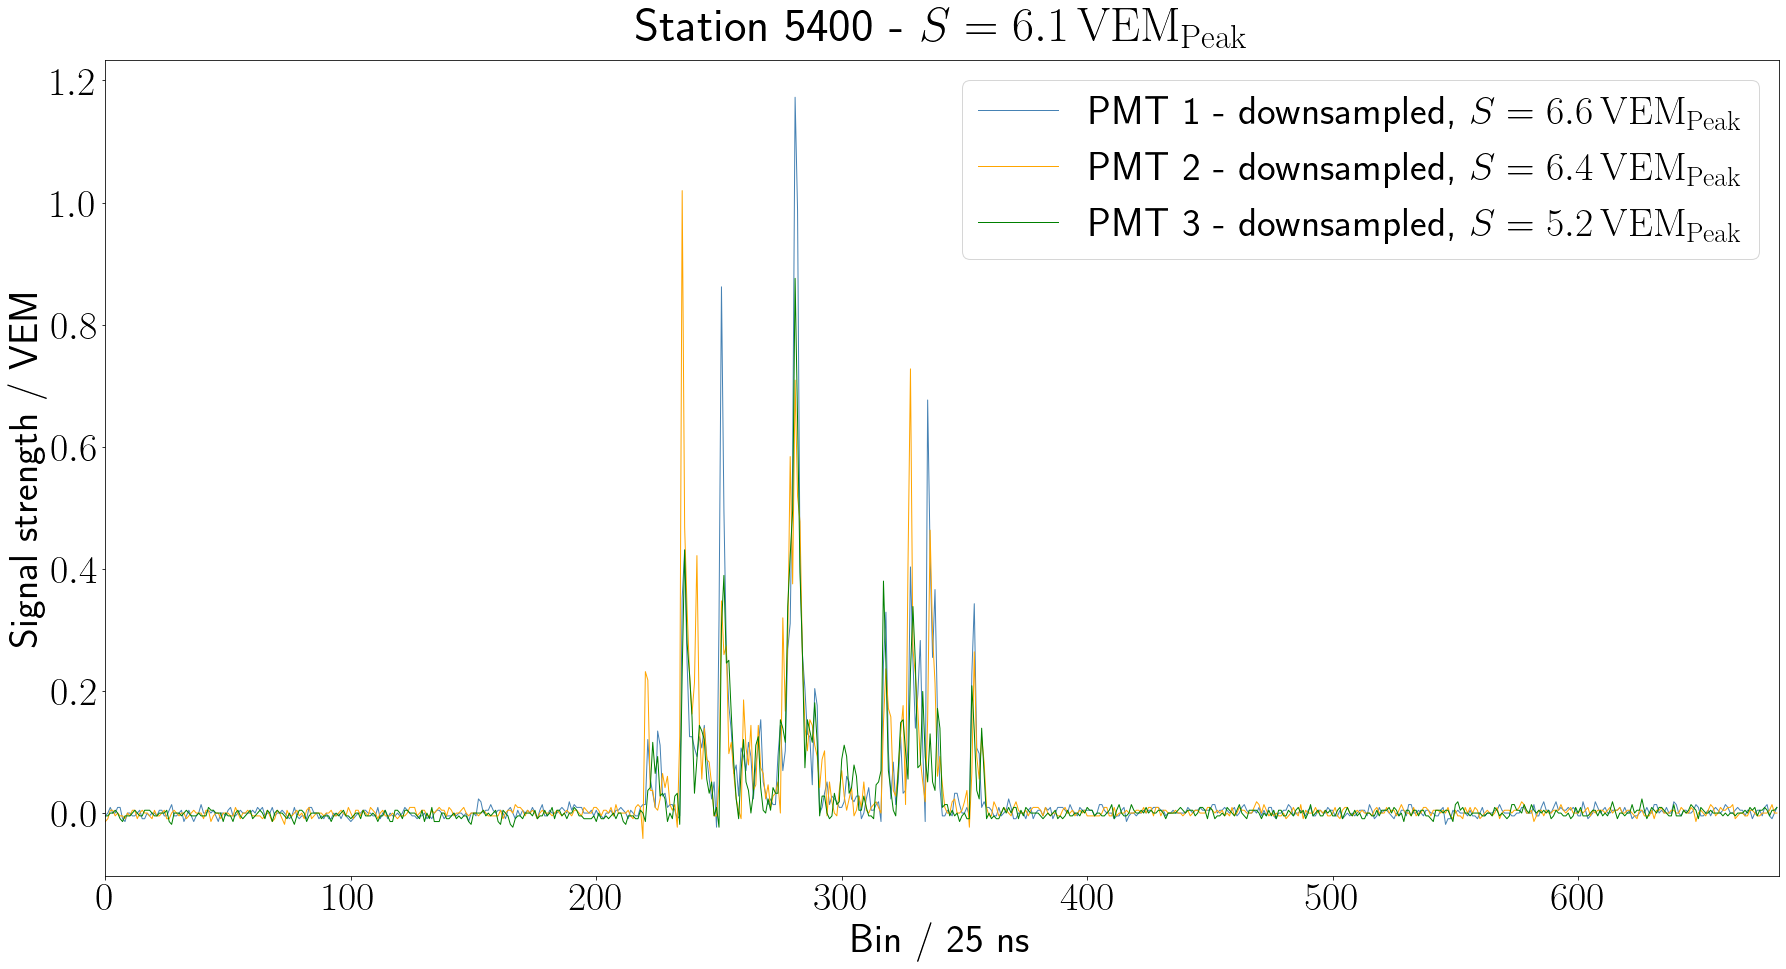
\includegraphics[width=\textwidth]{./plots/time_trace_UB.png}
		\caption{\textbf{UB time trace}}
		\label{fig:ub-time-trace}
	\end{subfigure}
	\caption{\textbf{(a)} A simulated signal as it would appear to UUB electronics. The ionizing particles originating in the extensive air shower hit the tank 
	around bin 660 ($\approx\SI{5.5}{\micro\second}$). \textbf{(b)} The same signal but filtered and downsampled to emulate UB electronics.}
	\label{fig:uub-ub-comparison}
\end{figure}

\subsection{Sliding window analysis \& Labelling}
\label{ssec:sliding-window-analysis}

As will become apparent in \autoref{chap:classical-triggers}, three of the four trigger algorithms operate by examining only a window of measurement info, rather
than evaluate the whole time trace as it is constructed in \autoref{sec:trace-building}. In a similar fashion, it is reasonable to assume neural networks do not 
need to receive the $3\,(\text{PMT})\cdot2048\,(\text{UUB bins}) = 6144$ input values from the entire trace to make an informed choice of whether or not a given
signal stems from an extensive air shower.

For this reason, samples from the time trace are drawn via a sliding window analysis. A number of $n_\text{bins}$ are extracted from the trace, to be analyzed 
by some classification algorithm. In order to not select the same information repeatedly, the window is moved by $n_\text{skip}$ bins forward and the process
can begin anew. Unless explicitly specified otherwise, the hyperparameters in this sliding window analysis are set as 

\begin{equation}
	\label{eq:sliding-window-analysis-hyperparameters}
	n_\text{bins} = 120, \qquad n_\text{skip} = 10.
\end{equation}

Whether or not a specific window contains signal from an extensive air shower - which is important for labelling data in the context of neural network training -
is a simple exercise. The modular approach in \autoref{sec:trace-building} allows to simply check for nonzero bins in the shower signal component of the trace.
In practice, upon creating a new combined trace, the first and last positive bin in the shower component are identified. This is e.g. visualized with dashed red 
lines in \autoref{fig:component_adding}. If any overlap - even just a single bin - exists between the sliding window and this signal region, the extracted window
is consequently labelled as signal. If this is not the case, the window is labelled as background.

Of course, quality cuts can be applied, and a decision to count a given trace window can be made individually. This is further discussed in 
\autoref{chap:neural-network-triggers}.